% !TeX root = ../main.tex
% Add the above to each chapter to make compiling the PDF easier in some editors.

\chapter{Related Work}\label{chapter:related_work}

\section{Emission Inventories}
Emission inventories are a estimation of emission fields
They serve two main purposes \parencite{CAMS-REG-v4}.
The first purpose is to 
Questions:
\begin{enumerate}
    \item what are the purpose of emission inventories
    \item what are Emission Inventories
    \item How are Emission Inventories generated
    \item what are the problems with bottom-up approaches for GHG emissions? 
    \subitem may miss
    \item what are typical approaches to top-down?
    \item what are the challenges in top-down approaches?
\end{enumerate}
Then go over to Benjis work who has shown that 
For this work, same assumptions as in Benjis work hold, i.e. background GHG emissions are ignored.

Bottom-up approaches estimate emission fluxes by multiplying emission sources with their activity \parencite{BU-vs-TD} (also cite inventories).
In contrast, top-down approaches start from measurements of GHG conecntrations and invert the transport of molecules to find the sources from which they emitted.
One example for a measurement network is MUCCnet \parencite{MUCCnet}.
Bottom-up approaches can miss emitters due to unknown datas whereas top-down approaches can be able to capture unknown emitters with measurements.
Furthermore, 
Bottom-up and top-down approaches show gaps in their esimtations which can largely be explained by temporal variability \parencite{BU-vs-TD}.


\section{Inverse Problems in GHG Emission Context}
How do top down approaches work?
What is the inverse problem?
Benji deonstrated use of compressed sensing.
Formulate the problem formulation for this thesis here.
Meaning, what are the constraints.
Background GHG emissions.
Assume linear forward model.

\section{Compressed Sensing}
Here, I should explain the general theory of compressed sensing.
Compressed sensing makes assumptions about the signal and forward model.
Generally, signals are assumed to be sparse in some basis.
If the forward model then fulfills certain criteria, reconstruction can be gurantueed.
Sparsity can be 

[Citations mssing]
The most basic algorithm to reconstruct a signal would be minimize the L0 norm of a signal.
The L0 norm is defined as the number of all non-zeros elements of a vector.
\begin{equation}
    min L0 of  s.t. y = Ax
\end{equation}
This problem is NP-hard and thus not practical in real world applications.
Instead, it can be shown that minimizing the L1 norm yields the same result as above under certain conditions.
\begin{equation}
    \min()
\end{equation}
This algorithm is known as basis pursuit (BP).

Basis pursuit is a very powerful algorithm, but assumes that measurements are ideal, i.e. not noisy.
Extensions of this algorithm exist that deal with noise.
This extension is called basis pursuit denoising (BPDN)
\begin{equation}
    \min()
\end{equation}
BPDN thus assumes that the noise level is known.

Furthermore, regularization teqhniues exist to also sovle comrpessed sensing problems, for instance the Lasso regularizer which assumes a Laplacian prior.
\begin{equation}
    Lasso
\end{equation}
It can be shown that BPDN is equivalent to the Lasso regularizer for a certain alpha.

For compressed sensing, signals must be sparse in some basis.
This can be done with overcomplete dictionaries, transforms, etc.
Common way is wavelet transform or discrete cosine transform.

Recent developments make use of generative models for low dimensional representations which can be interpreted as sparse maps.
This samples can be generated and thus represented with only few dimensions.

There are three main approaches to alleviate sparsity constraint.
1) transforms, such as Wavelet
2) only searching for unknown emissions and take esimtations as basis
3) Deep learning based approaches


\section{Generative Models for Compressed Sensing}
Here I want to give an overview of generative models can be used for compressed sensing.
I should use the review as reference and give a short summary.

The field of medical imaging has made advancements in the inverse problems using deep learning.
A review of different deep learning approaches for CS is given in \parencite{ReviewCSUsingAI}
They mention Bora et al \parencite{CSUsingAI}.
Their approach has the limitation that the reconstruction is constrained to the range of the generator.
This, however, can improved by also taking into account other things: \parencite{SparseCSUsingAI}.

Make a diagram of how the generative models are used.
\begin{figure}[h!]
    \centering
    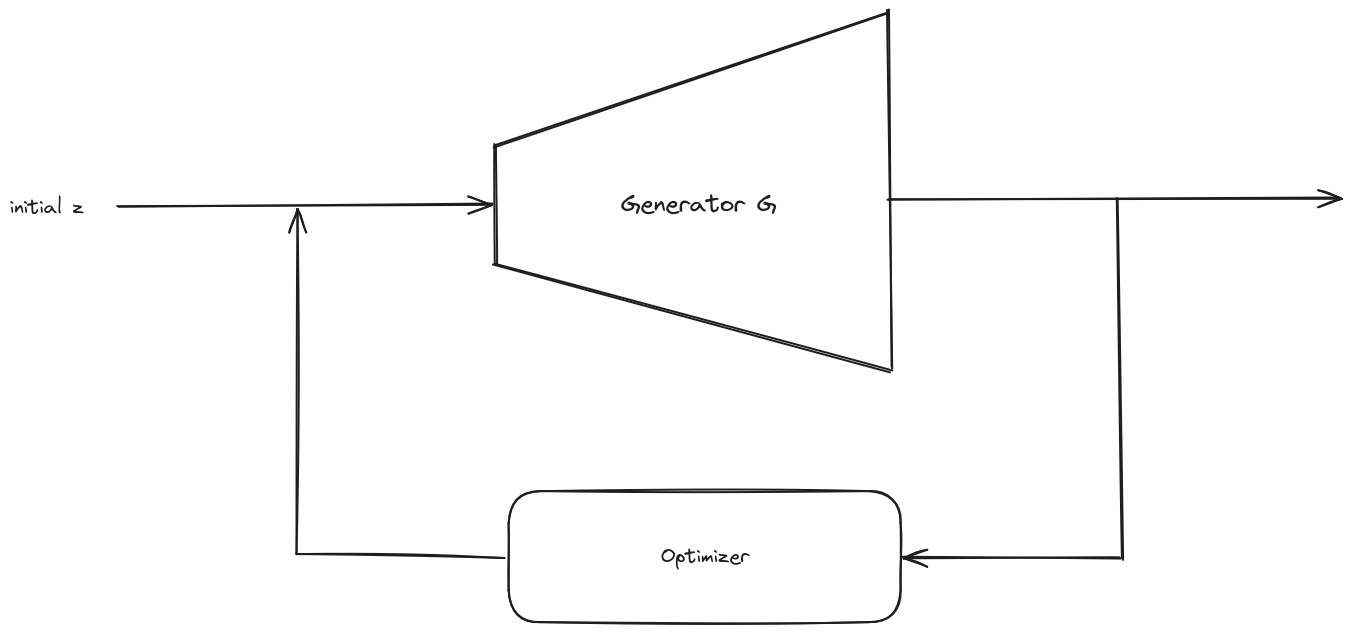
\includegraphics[width=\textwidth]{figures/02_related_work/bora_et_al.png}
    \caption{Bora et al Paper}
\end{figure}

Assuming a linear forward model $y = Ax + \epsilon$ with $A \in \mathbb{R}^{m \times n}$
Given is a generator $G: \mathbb{R}^d \to \mathbb{R}^n$ and the compressed sensing problem.
Solve the following minimization problem:
\begin{equation}
    z^* = \arg\min_{z}{\left( \norm{A G(z) - y}_2^2 + \alpha R(z) \right)}
\end{equation}
An improvements is made by to further consider sparse deviations from the generated emission fields:
\begin{equation}
    z^* = \arg\min_{z, s}{\left(\norm{s}_1 + \lambda \norm{A \left( G(z) + s \right) - y}_2^2 \right)}
\end{equation}

\section{Generative Models}
There are three main kinds of modern successful generative models in the context of sample generation.
These models are not limited to image generation only.
There are variational autoencoders, generative adverserial networks, and score based models.
Both VAEs and GANs generate samples from lower dimensionional noise.
Score based models generate samples by denoising previous samples, starting from noise.
The noise and generated samples thus have same dimensions for score based models.
Due to this, score based models are not directly applicable with the method from \parencite{CSUsingAI}.
However, alternative approaches for score based models exist, which are not explored here.
While GANs show higher quality generation for many different domains, GANs are difficult to train as the objectives can get very unstable.
Therefore, for this thesis, VAE is chosen as the appropriate type of generative model

\section{Contributions}
The point of this work is not to investigate whether compressed sensing theory can be applied in the context of 
This has been investigated by prior work, like Benjis.
The point of this thesis is to investigate whether generative models can be applied.

Is the model able to generalize beyond the trianing data?
Is the model able to reconstruct emitters that are not covered in the emission inventories? 
What is a good dimension for the lower dimensional space?

Mention the rough constributions of this work:
\begin{enumerate}
    \item trained VAE for emission inventories of European cities
    \item demonstrated the applicability of generative models in the context of inverse models for top-down approaches
\end{enumerate}
